\subsubsection{Strategien zur Fehlerbehebung und Optimierung}
\label{chap:Strategien zur Fehlerbehebung und Optimierung}

Im vorherigen Kapitel \ref{chap:Herausforderungen bei der Übernahme und Anpassung} wurde bereits gezeigt, dass die Implementierung des \ac{c-ep} sinnvolle Gewichte für \(\vec{d}=(0.8,0.8,0.8)\) findet. Da die Aktivierungsfunktion in Annäherung an \(\rho(x)=0\) bzw. \(\rho(x)=1\) eher große Werte \(x\) benötigt (\(\rho(4.5952)\approx0.99\)), müssen die Zustände des Netzwerks bzw. die Gewichte entsprechend große Werte annehmen, um die Zielwerte \(0\) bzw. \(1\) abzubilden. Die Konvergenz der Gewichte ist für diese Zielwerte auch nicht möglich, weshalb das \ac{c-ep} in diesem Fall die Gewichte endlos vergrößert bzw. verkleinert. Eine mögliche Lösung hierfür könnte das Austauschen der Aktivierungsfunktion gegen die sog. "`ReLU"'-Funktion (\(R(x)=max(x,0)\)) sein, welche linear im Wertebereich \(x>0\) verläuft. Beim Anwenden auf das \ac{hnn} führt ReLU aber zu Problemen, da das Netzwerk damit nicht konvergiert und somit unbrauchbare Werte ausgibt. In Anlehnung an \cite[vgl. S. 31]{Ernoult2020} kann die bereits genutzte Aktivierungsfunktion \(\rho(x)=\frac{1}{1+e^{-x}}\) skaliert werden, um ihre S-Kurve zu stauchen und damit die Annäherung an \(0\) bzw. \(1\) zu vereinfachen. Die abgewandelte Funktion \(\rho(x)=\frac{1}{1+e^{-4x}}\) ist in Abbildung \ref{fig:Graph der skalierten Aktivierungsfunktion} dargestellt.

\begin{figure}[h]
  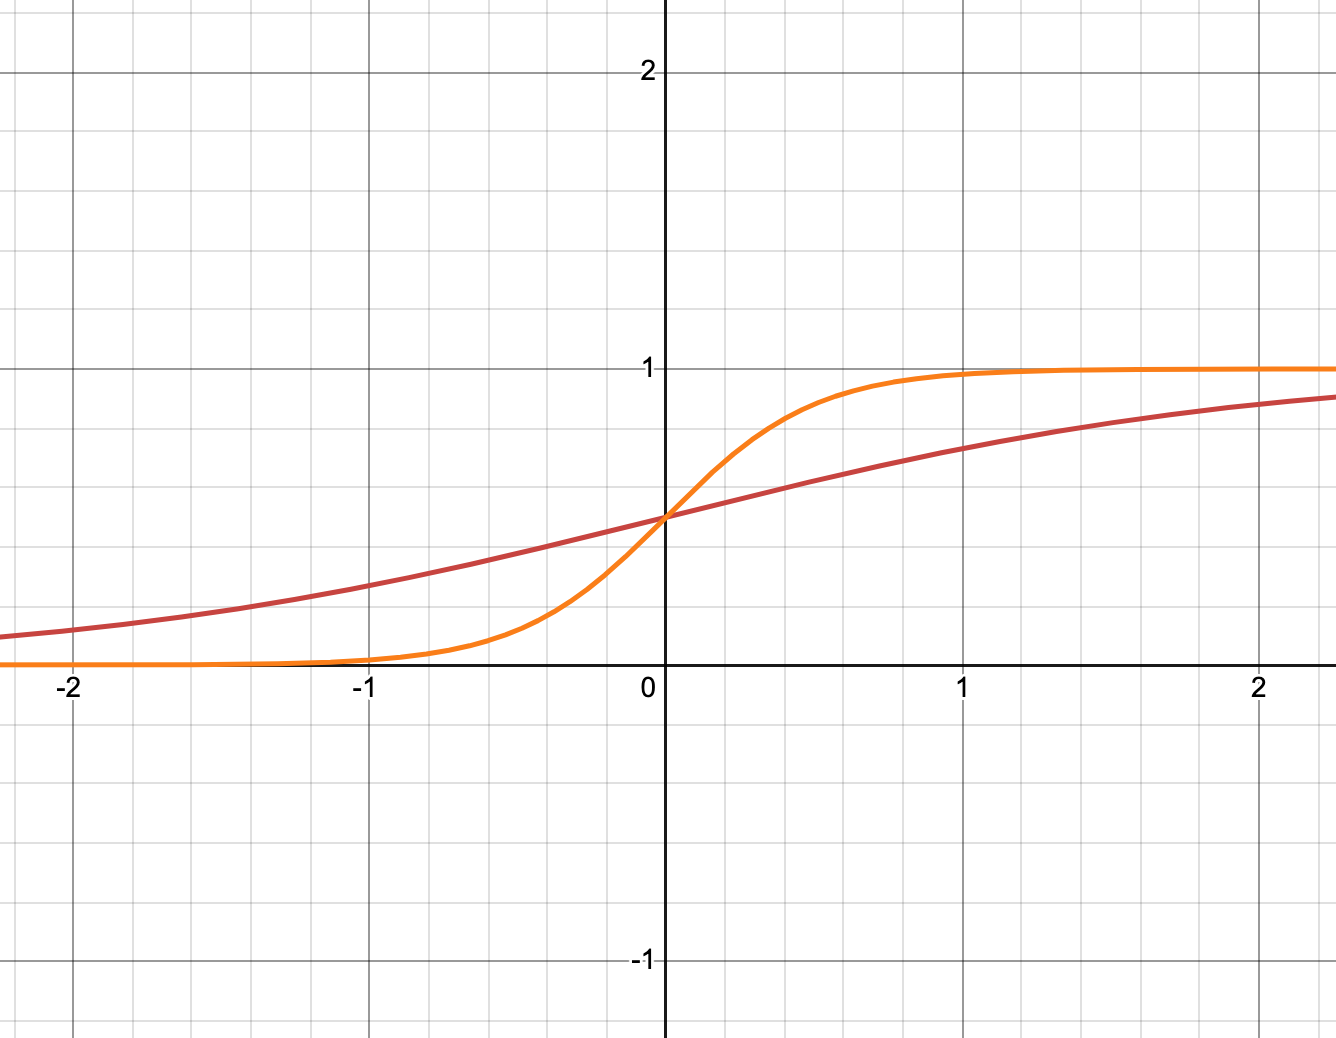
\includegraphics[width=0.5\textwidth]{abbildungen/sigmoid_funktion_skaliert.png}
  \caption{Graph der Aktivierungsfunktion (rot) und der skalierten Variante \(\rho(x)=\frac{1}{1+e^{-4x}}\) (orange). Quelle: \textit{Eigene Darstellung}}
  \label{fig:Graph der skalierten Aktivierungsfunktion}
\end{figure}

Mit den Parametern \(\beta=1\) und \(\eta=1\) findet das \ac{c-ep} mit dieser skalierten Aktivierungsfunktion und den Zielwerten \(\vec{d}=(0,0,0)\) Gewichte, welche die Ausgabe \(\vec{y}\approx(0.14,0.14,0.16)\) erzeugen, damit zwar in die Nähe der Zielwerte gelangen aber diese noch immer drastisch verfehlen. Werden aber Zielwerte abseits der Grenzwerte \(0\) bzw. \(1\) beispielsweise \(\vec{d}=(0.2,0.5,0.8)\) betrachtet, so werden Gewichte gefunden, mit denen ein Fehler von \(C(y)<0.001\) erreicht wird. Ein weiterer Durchlauf mit den Zielwerten \(\vec{d}=(0.3,0.4,0.7)\) führt zu einem Fehler der Größenordnung \(10^{-6}\) in unter zehn Epochen. Aufgrund dieser Verbesserungen wird mit der skalierten Aktivierungsfunktion weitergearbeitet.
